\documentclass[fr]{../../../eplnotes}

\usepackage{../../../eplunits}

\newcommand{\hati}{\hat{\imath}}
\newcommand{\hatj}{\hat{\jmath}}
\newcommand{\hatk}{\hat{k}}

\newcommand{\norm}[1]{\left\lVert#1\right\rVert}
\setcounter{equation}{1} % pour des raisons obscures,eil commençait à 0

\hypertitle{Mécanique}{1}{FSAB}{1201}
{Mattéo Couplet}
{Roland Keunings}[
\paragraph{Remarque}
Ce document a pour objectif de rassembler les démonstrations importantes du cours en vue de l'examen. Il suppose une compréhension préalable de la matière et ne fait office ni de synthèse, ni de syllabus.
]

%\begin{document}


\section{Cinématique du mouvement circulaire}
\begin{center}
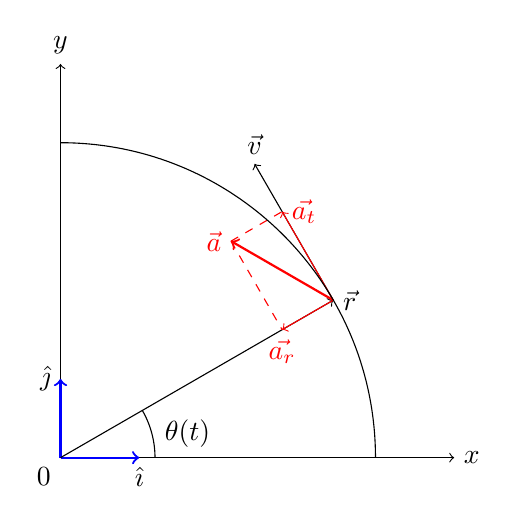
\begin{tikzpicture}[x=1cm,y=1cm]

    \def\R{4}
    \def\angle{30}
    \def\Al{1.5}
    \def\Vl{2}
    \def\UnitArcRadius{1.2}

    \coordinate (O) at (0,0);
    \coordinate (Xmax) at (5,0);
    \coordinate (Ymax) at (0,5);
    \coordinate (P) at ({\R*cos(\angle)},{\R*sin(\angle)});
    \coordinate (V) at ({(\R*cos(\angle)) + (\Vl*cos(\angle+90))},{(\R*sin(\angle)) + (\Vl*sin(\angle+90))});
    \coordinate (A) at ({(\R*cos(\angle)) + (\Al*cos(\angle+120))},{(\R*sin(\angle)) + (\Al*sin(\angle+120))});
    \coordinate (A1) at ({(\R*cos(\angle)) + (\Al*cos(\angle+120)) + (\Al*0.5*cos(\angle))},{(\R*sin(\angle)) + (\Al*sin(\angle+120)) + (\Al*0.5*sin(\angle))});
    \coordinate (A2) at ({(\R*cos(\angle)) + (\Al*cos(\angle+120)) + (\Al*cos(\angle)*cos(\angle+270))},{(\R*sin(\angle)) + (\Al*sin(\angle+120)) + (\Al*cos(\angle)*sin(\angle+270))});
    
    
    \draw[->]            (O) -- (Xmax); 
    \draw[->,blue,thick] (O) -- (1,0);
    \draw[->]            (O) -- (Ymax);
    \draw[->,blue,thick] (O) -- (0,1);
    \draw[->]            (O) -- (P);
    \draw[->]            (P) -- (V);
    \draw[->,red,thick]  (P) -- (A);
    \draw[->,red]        (P) -- (A1);
    \draw[->,red]        (P) -- (A2);
    \draw[red,dashed]    (A) -- (A1);
    \draw[red,dashed]    (A) -- (A2);

    \draw (\R,0) arc (0:90:\R);
    \draw (\UnitArcRadius,0)  arc (0:\angle:\UnitArcRadius);

    \draw (Xmax) node[right]{$x$};
    \draw (Ymax) node[above]{$y$};
    \draw (O)    node[below left]{$0$};
    \draw (1,0)  node[below]{$\hat{\imath}$};
    \draw (0,1)  node[left]{$\hat{\jmath}$};
    \draw (\UnitArcRadius,0) node[above right]{$\theta(t)$};
    \draw (P)    node[right]{$\vec{r}$};
    \draw (V)    node[above]{$\vec{v}$};
    \draw (A)    node[red,left]{$\vec{a}$};
    \draw (A1)   node[red,right]{$\vec{a_t}$};
    \draw (A2)   node[red,below]{$\vec{a_r}$};
    
\end{tikzpicture}
\end{center}

\label{sec:mouv_circ}
Soit un corps ponctuel en mouvement circulaire. On note son vecteur position $\vec{r}$, tel que $\norm{\vec{r}} = R$, où $R$ est le rayon du cercle dans lequel il se meut. On place un repère orthonormé au centre dudit cercle, et on définit $\theta$ comme l'angle que forme $\vec{r}$ dans ce système. On a alors
\[ \vec{r} = R (\cos\theta \ \hati +\sin\theta \ \hatj) \]
On sait que la vitesse de l'objet est la dérivée de sa position par rapport au temps :
\begin{align*}
    \vec{v} &= \fdif{\vec{r}}{t} = R(-\dot{\theta} \sin\theta\ \hati + \dot{\theta} \cos\theta\ \hatj) \\
    \norm{\vec{v}} &= R \sqrt{(-\dot{\theta} \sin\theta)^2 + (\dot{\theta} \cos\theta)^2} = \dot{\theta} R \tag{\theequation}\label{speed}
\end{align*}

L'accélération est la dérivée de sa vitesse par rapport au temps :
\begin{align*}
    \vec{a} = \fdif{\vec{v}}{t} = R \left( \left(-\ddot{\theta} \sin\theta \ - \dot{\theta}^2 \cos\theta \right) \hati + \left(\ddot{\theta} \cos\theta - \dot{\theta}^2 \sin\theta\right) \hatj \right)
\end{align*}

On définit deux vecteurs unitaires, un radial et un tangentiel, de la sorte
\begin{alignat*}{3}
    & \vec{e_r} &&= \cos\theta \hati + \sin\theta \hatj &&\qquad \text{et $\vec{e_r} \parallel \vec{r}$} \\
    & \vec{e_t} &&= -\sin\theta \hati + \cos\theta \hatj && \qquad \text{et $\vec{e_t} \parallel \vec{v}$}
\end{alignat*}

Pour obtenir l'accélération radiale (vers le centre du cercle), on projette $\vec{a}$ sur $-\vec{e_r}$ (ce vecteur unitaire pointe vers l'extérieur, d'où le signe) :
\begin{align*}
    a_r &= - \vec{a} \cdot \vec{e_r} \\
    &= R \left(\ddot{\theta} \cos\theta\sin\theta + \dot{\theta}^2 \cos^2\theta - \ddot{\theta} \sin\theta\cos\theta + \dot{\theta}^2 \sin^2\theta\right) \\
    &= \dot{\theta}^2 R \stackrel{\eqref{speed}}{=} \frac{v^2}{R} 
\end{align*}

On obtient ensuite l'accélération tangentielle (tangent à la trajectoire) en projetant $\vec{a}$ sur $\vec{e_t}$ :
\begin{align*}
    a_t &= \vec{a} \cdot \vec{e_t} \\
    &= R \left( \ddot{\theta} \sin^2\theta + \dot{\theta}^2 \cos\theta\sin\theta + \ddot{\theta}\cos^2\theta - \dot{\theta}^2\sin\theta\cos\theta\right) \\
    &= \ddot{\theta} R \stackrel{\eqref{speed}}{=} \dot{v}
\end{align*}

En résumé, on retient les trois relations suivantes dans un mouvement circulaire
\[ \norm{\vec{v}} = \dot{\theta}R \qquad a_r = \frac{\norm{\vec{v}}^2}{R} \qquad a_t = \fdif{\norm{\vec{v}}}{t} \]

\section{Énergie potentielle gravitationnelle}
\subsection{Cas général}
On a la loi de gravitation universelle de Newton
\[ F_g = \frac{Gmm_E}{r^2} \]
où $m$ est la masse du corps en question, $m_E$ la masse de la Terre, $r$ la distance entre le corps et le centre de la Terre et $G = \SI{6.67e-11}{\cubic\meter\per\kilogram\per\second\squared}$, la constante gravitationnelle.\\
Le travail pour aller d'un point $P_1$ à $P_2$ vaut
\[
    W = \int_{P_1}^{P_2} \vec{F} \cdot \dif \vec{l} = -Gmm_E \int_{P_1}^{P_2} \frac{1}{r^2} \dif l \cos\theta
\]
On remplace $\dif l \cos\theta = \dif r$ :
\begin{align*}
    W &= -Gmm_E \int_{r_1}^{r_2} \frac{1}{r^2} \dif r \\
    &= -Gmm_E \left[ \frac{-1}{r} \right] _{r_1}^{r_2} \\
    &= Gmm_E \left( \frac{1}{r_2} - \frac{1}{r_1} \right)
\end{align*}

On définit l'énergie potentielle $U$ telle que $W_\mathrm{grav} = U_1 - U_2$ ; dès lors
\[ U_\mathrm{grav} = \frac{-Gmm_E}{r} \]

On remarque qu'à une distance infinie de la Terre, $U = 0$. L'énergie potentielle est donc strictement négative, strictement croissante avec la distance, et nulle à l'infini.

\subsection{Au voisinage de la Terre}
On aimerait approcher la valeur de l'énergie potentielle gravitationnelle pour des altitudes $y$. On pose $r = R_E + y$ la distance par rapport au centre de la Terre ; on remplace dans l'expression de l'énergie potentielle 
\[ U = \frac{-Gmm_E}{R_E + y} = \frac{-Gmm_E}{R_E(1+y/R_E)} \]
L'accélération terrestre au sol vaut $g = \frac{Gm_E}{R_E^2}$ ; on replace donc
\[ U = -mgR_E \frac{1}{1+y/R_E} \]
On pose $x = \frac{y}{R_E} \ll 1$ car on est à basse altitude. On définit la fonction $f(x) = \frac{1}{1+x}$ et on développe son polynôme de Taylor :
\[ f(x) \approx f(0) + f'(0) (x - 0) + \text{HOT} \]
HOT signifie ``higher order terms''. Puisque $x$ est petit, on les ignore, ce qui nous donne
\[ f(x) \approx 1 - x \]

En remplaçant dans l'expression de $U$, on obtient
\[ U = -mgR_E + mgy \]
Si on définit l'énergie potentielle comme nulle à la surface de la Terre, ($U(y = R_E) = 0$), l'expression devient
\[ U = mgy \qquad \text{tant que $y \ll R_E$} \]

\section{Satellites : orbites circulaires}
Soit un satellite en orbite circulaire autour de la Terre, de sorte que la seule force s'appliquant sur lui soit l'attraction terrestre. Par la seconde loi de Newton,
\[ \sum F = \frac{Gmm_E}{r^2} = ma \]
Or, l'accélération en question n'est rien d'autre que l'accélération centripète qui permet au satellite de rester en mouvement circulaire uniforme. Comme vu en section \ref{sec:mouv_circ}, l'accélération radiale est donnée par
\[ a_r = \frac{v^2}{r} \]
Dès lors, on a la relation 
\[ \frac{Gmm_E}{r^2} = \frac{mv^2}{r} \]
à partir de laquelle on trouve la vitesse du satellite à une distance $r$ du centre de la Terre :
\[ v = \sqrt{\frac{Gm_E}{r}} \]
Notons qu'elle ne dépend pas de la masse du satellite. Si le satellite se meut à une vitesse inférieure ou supérieure, la trajectoire ne sera plus circulaire.\\
On peut maintenant aisément déterminer la période de révolution du satellite
\[
    T = \frac{2\pi R}{v} = \frac{2\pi r^{3/2}}{\sqrt{Gm_E}}
\]

Calculons l'énergie totale que possède un satellite en orbite circulaire
\begin{align*}
    E &= K+U \\
    &= \frac{1}{2}mv^2 + \left( -\frac{Gmm_E}{r} \right) \\
    &= -\frac{Gmm_E}{2r} 
\end{align*}

Cette énergie est donc strictement croissante et tend vers zéro à l'infini.

\section{Vitesse de libération}

\subsection{De la Terre}
On souhaite calculer la vitesse minimale nécessaire pour envoyer un objet dans l'espace tel qu'il ne retombe jamais sur Terre. On applique la loi de conservation de l'énergie mécanique :
\[ K_1 + U_1 = K_\infty + U_\infty \]
À une distance infinie de la Terre, l'énergie potentielle est nulle par convention. On suppose qu'à l'infini, il n'a plus d'énergie cinétique (car on veut la vitesse \emph{minimale}) :
\[
    \frac{1}{2}m v_l^2 + \left( -\frac{Gmm_E}{r_E} \right) = 0 \Rightarrow v_l = \sqrt{\frac{2Gm_E}{r_E}}
\]
Pour la Terre, cette vitesse vaut à peu près \SI{40200}{\kilo\meter\per\hour}.

\subsection{D'étoiles plus massives} 
Pour une étoile de rayon $R$ et de masse $M$, la formule de la vitesse de libération ne change pas
\[ v = \sqrt{\frac{2GM}{R}} \]
Dans des cas extrêmes, le rapport masse-rayon (c'est-à-dire la densité) est tellement grand que la vitesse de libération excède la vitesse de la lumière. Dans ce cas, on parle d'un trou noir. Pour une étoile de masse $M$, le rayon maximal qu'elle peut atteindre avant de devenir un trou noir s'appelle \emph{rayon de Schwarzschild} et s'obtient en replaçant la vitesse de libération par $c$, la vitesse de la lumière :
\[ R_\mathrm{S} = \frac{2GM}{c^2} \]
\emph{Attention} : en réalité, la mécanique newtonienne telle que nous la connaissons n'est plus d'application à des vitesses aussi élevées ; on doit alors se référer à la mécanique relativiste. Dans ce cas précis, remplacer $v$ par $c$ fonctionne par compensation d'erreur.

\section{Mouvement périodique}

Un corps effectue un mouvement périodique si la force de rappel est directement proportionnelle à son déplacement.

\subsection{Ressort}
Un ressort idéal obéit à la loi de Hooke 
\[ F_x = -kx \]
où $k$ est appelée la constante de raideur ou constante de Hooke. En vertu de la seconde loi de Newton, on transforme l'équation
\[ \frac{\dif^2 x}{\dif t^2} = -\frac{k}{m} x \]
C'est une équation différentielle du second degré en $x(t)$. La solution générale de ce type d'équation est
\[ x(t) = A \cos(\omega t + \phi) \]
où $A$ est l'amplitude de l'oscillation, $\omega$ la fréquence angulaire et $\phi$ le déphasage. Si on injecte cette expression dans l'équation différentielle, on trouve immédiatement $\omega$ :
\[ -\omega^2 A \cos(\omega t + \phi) = -\frac{k}{m} A \cos(\omega t + \phi) \ \Rightarrow \ \omega = \sqrt{\frac{k}{m}} \]

Deux données sont nécessaires pour déterminer $A$ et $\phi$. Classiquement, on utilisera le déplacement initial $x_0$ et la vitesse initiale $v_0$. On déduit les formules suivantes (les détails sont laissés au lecteur) :
\[ \phi = \arctan \left(-\frac{v_0}{\omega x_0} \right) \qquad A = \sqrt{x_0^2 + \frac{v_0^2}{\omega^2}} \]

\subsection{Pendule simple}
Dans le pendule simple, la force de rappel (qui est la force tangente à la trajectoire de la masse) est proportionnelle au sinus de l'angle que l'objet forme avec la verticale :
\[ F_t = -mg\sin\theta \]
Le mouvement n'est donc pas strictement périodique simple. En revanche, pour des petits angles, on a $\sin x \approx x$. Supposons que cette différence soit négligeable (attention : tout ce qui suit à partir de maintenant est faux pour des grands angles !) :
\[ F_t = -mg\theta = -mg\frac{x}{L} = -\frac{mg}{L} x \]
La constante de force est donc $k = mg/L$. On en déduit la fréquence angulaire du pendule simple
\[ \omega = \sqrt{\frac{k}{m}} = \sqrt{\frac{g}{L}} \]
Notons que $\omega$ ne dépend pas de la masse de l'objet oscillant.

\end{document}
